\documentclass{article}
\usepackage{listings}
\usepackage{geometry}
\usepackage{graphicx}
\usepackage{amssymb}
\usepackage{amsmath}
\usepackage{hyperref}
\usepackage[english]{babel}
\usepackage{amsthm}
\usepackage{mathrsfs}
\usepackage{blindtext}
\usepackage{titlesec}
\usepackage{algorithm}
\usepackage{algpseudocode}
\usepackage[utf8]{inputenc}
\usepackage{fancyhdr}
\usepackage{braket}
\usepackage{mathtools}


\usepackage[backend=bibtex, style=numeric]{biblatex}

\usepackage[english]{babel}

\usepackage{filecontents}
\usepackage{algorithmicx}

\begin{filecontents*}{\jobname.bib}

% Add the references here

@book{ideals-varieties-algorithms,
    author = {{D. A. Cox, J. Little, and D. O'Shea}},
    title = {Ideals, Varieties, and Algorithms (third edition)},
    publisher = {Springer-Verlag New-York},
    year = {2007}
}


\end{filecontents*}

\addbibresource{\jobname.bib}

\newtheorem{theorem}{Theorem}[section]
\newtheorem{corollary}{Corollary}[theorem]
\newtheorem{lemma}{Lemma}[section]
\newtheorem{definition}{Definition}[section]
\newtheorem{proposition}{Proposition}[section]
\newtheorem{example}{Example}[section]
\newtheorem{property}{Property}[section]
\newtheorem{remark}{Remark}[section]

\title{PSFPN - Gröbner bases in two variables}
\begin{document}
%\geometry{legalpaper, margin=2cm}
\setlength{\parindent}{0pt}


\DeclarePairedDelimiter\ceil{\lceil}{\rceil}
\DeclarePairedDelimiter\floor{\lfloor}{\rfloor}

\rfoot{\thepage}


\begin{center}
    \textbf {
        \vspace*{1mm}
        \vspace*{1mm}
         \noindent\rule[0.3\baselineskip]{\textwidth}{1pt}
        \LARGE{PSFPN - Gröbner bases of two variables\\}
}
         \noindent\rule[0.3\baselineskip]{\textwidth}{1pt}
         \vspace{5mm}
        \begin{center}
    		\begin{figure*}[!ht]
    			\centering{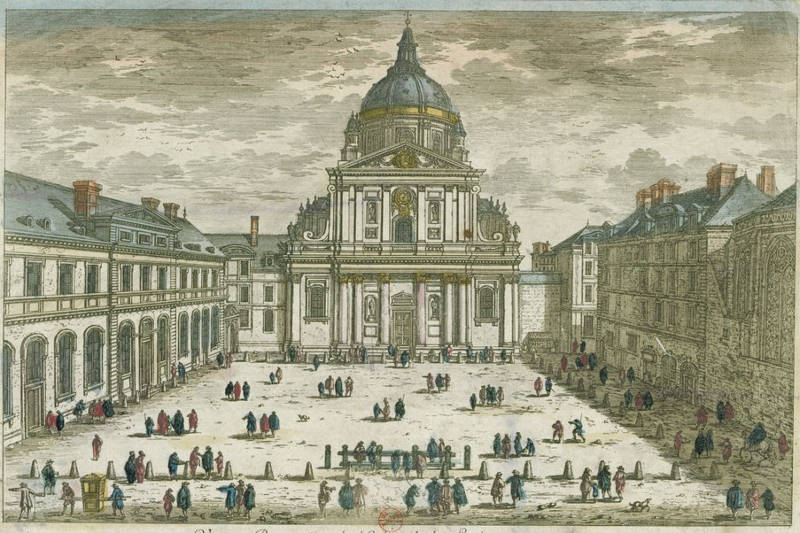
\includegraphics[scale=0.5]{C.png}}
    	    \end{figure*}
    	\end{center}
        \vspace*{15mm}
        \large {Auguste WARME-JANVILLE, Alan PULVAL-DADY \\ }

\end{center}

\newpage
     
\section*{Introduction}

Given $f_{1}=0,\dots,f_{r}=0$ where $f_{1},\dots,f_{r}$ are polynomials in $x$ and $y$ with coefficients in a field $\mathbb{K}$, we are interested in computing solutions of the systems. A Gröbner basis of the ideals $<f_{1},\dots,f_{r}>$ is a set of generators with advantageous properties for solving the system mentioned above and also to guess the belonging or not of a polynomial to the ideal above. Studying the structures of these bases is, therefore, a valuable approach for efficiently solving such systems. \\
It is known that when the system has a finite number of solutions, the associated Gröbner bases under the lexicographical order contain at least two non-zero polynomials that can be distinguished : (1) one exclusively in terms of y and (2) another where the leading term is a power of x. \\
The objective of this project is to investigate the structure of these bases. \\
To accomplish this, we first examined the construction of a Gröbner basis and then established the existence of polynomials (1) and (2). Subsequently, we explored the structure of the intersection of two Gröbner bases with specific properties(link). \\
Finally, we extended our analysis to the structure of the intersection of N Gröbner bases. \\ \\

\textbf{We would like to extend our sincere appreciation to our supervisor Jeremy Berthomieu from the LIP6 PolSys  team for his invaluable guidance and expertise throughout this project.}

\newpage      

\section{Ideals}

\begin{definition}[Ideal]
    Let $(R, +, \cdot)$ be a ring. $I$ is an ideal of $R$ if : 
    \begin{itemize}
        \item $I$ is a subgroup of $(R, +)$
        \item For all $x \in R$ and $i \in I$, $x \cdot i \in I$
    \end{itemize}
\end{definition}

We will assume that all the rings we work on are commutative. 

\begin{definition}[Principal Ideal]
    An ideal $I$ of a ring $R$ is called principal if it is generated by a single element $f$ of $R$, \textit{i.e.}
    \begin{displaymath}
        I = \{f \cdot a \mid \forall a \in R\}
    \end{displaymath}
    Such an ideal will be denoted $\langle f \rangle$.
\end{definition}

We will also define the intersection and the sum of two ideals, as they will be used later on.


\begin{definition}
    Let $I_{1} = \langle f_{1}, ..., f_{r} \rangle$ and  $I_{2} = \langle g_{1}, ..., g_{s} \rangle $ two ideals of $R$. 
    \begin{displaymath}
        I_{1} + I_{2} = \{f + g \mid f \in I_{1}, g \in I_{2}\} = \langle f_{1}, ..., f_{r}, g_{1}, ..., g_{s} \rangle 
    \end{displaymath}
\end{definition}

\begin{definition}
    Let $I_{1}, I_{2}$ two ideals of $R$. 
    \begin{displaymath}
        I_{1} \cdot I_{2} = \langle f_{1}f_{2} \mid f_{1} \in I_{1}, f_{2} \in I_{2} \rangle
    \end{displaymath}
\end{definition}

\begin{proposition}
    Let $I_{1}, I_{2}$ two ideals of $R$. 
    \begin{displaymath}
        I_{1} \cdot I_{2} \subseteq I_{1} \cap I_{2}
    \end{displaymath}
\end{proposition}

\begin{proof}
    Let $f \in I_{1} \cdot I_{2}$. By definition, $f \in I_{1}$ as the operator ($\cdot$) is absorbant. Same goes for $I_{2}$, hence the result.
\end{proof}

\section{Monomial orderings}

When studying polynomials of only one variable, the order of the monomials is straightforward : we implicitely assume that $1 < x < x^{2} < ...$. If we rise the number of variables we study, we can still sort all the powers of one variable with each other, but how do we manage monomials that are products of more than one variable ? There are many ways to handle this order problem. This is why we'll introduce \textit{monomial orderings}. 

\begin{definition}[Monomial ordering]\label{def:monomial-order}
    A monomial ordering $\prec$ on $\mathbb{K}[x, y]$ is any ordering on the monomials $x^{i}y^{j}$ : 
    \begin{itemize}
        \item $\prec$ is a total order
        \item If $w \neq 1$ is a monomial of $\mathbb{K}[x, y]$ then $1 \prec w$
        \item If $w$ is a monomial of $\mathbb{K}[x, y]$ and if $u \prec v$ then $uw \prec vw$
    \end{itemize}
\end{definition}

\begin{definition}[Lexicographic order]\label{def:lexicographic-order}
    The lexicographic order $\prec_{lex}$ is the monomial order over $\mathbb{K}[x, y]$ defined as : 
    \begin{displaymath}
        \forall i \in \mathbb{N}, y^{i} \prec_{lex} x
    \end{displaymath}
\end{definition}

\begin{proposition}
    For all $i, j, k, l \in \mathbb{N}$, $x^{i}y^{j} \prec_{lex} x^{k}y^{l}$ if and only if one of the following conditions are satisfied : 
    \begin{itemize}
        \item $i < k$
        \item $i = k$ and $j < l$
    \end{itemize}
\end{proposition}

\begin{proof}
    $\Rightarrow$ \newline
    $y^{m} \prec_{lex} x^{m}$ \ref{def:lexicographic-order} \newline
    $y^{m+l} \prec_{lex} y^{l}x^{m}$ \ref{def:monomial-order} \newline
    $x^{i}y^{m+l} \prec_{lex} y^{l}x^{m+i}$ \ref{def:lexicographic-order} \newline
    $j = m+l$ $ k = m + i$ and we have that $m+i>i \Rightarrow k > i$ \newline
    $\Leftarrow$ Let suppose that we have $i<k$ We can then write 
    \newline
    $x^{i}\prec_{lex} x^{k}$ \ref{def:lexicographic-order} \newline
    $x^{i}y^{j}\prec_{lex} 
    x^{k}y^{j}$ \ref{def:monomial-order}
    \newline
    $x^{k}y^{j} \prec_{lex} x^{k+1}y^{j} $ \ref{def:lexicographic-order}, \ref{def:monomial-order}
    \newline
    $x^{k}y^{j}y^{w} \prec_{lex} x^{k+1}y^{j}y^{w} $ \ref{def:monomial-order}
    \newline
    $x^{i}y^{j}\prec_{lex} 
    x^{k}y^{j}\prec_{lex} x^{k'}y^{l} $ \ref{def:monomial-order}
    \newline
    $x^{i}y^{j}\prec_{lex} x^{k'}y^{l} $
    
    
\end{proof}

\begin{definition}[DRL order]
    The DRL (Degree Reverse Lexicographic) order $\prec_{drl}$ is a monomial order over $\mathbb{K}[x, y]$ defined as : 
    \begin{itemize}
        \item $y \prec_{drl} x$
        \item For all $i, j, k, l \in \mathbb{N}$, $x^{i}y^{j} \prec_{drl} x^{k}y^{l}$ if and only if one of the following conditions are satisfied : 
        \begin{itemize}
            \item $i + j < k + l$.
            \item $i + j = k + l$ and $j > l$.
        \end{itemize}
    \end{itemize}
\end{definition}

\begin{example}
    The first monomials for the DRL order appearing in $\mathbb{K}[x, y]$ are : \\
    $1 \prec_{drl} y \prec_{drl} x \prec_{drl} y^{2} \prec_{drl} xy \prec_{drl} x^{2} \prec_{drl} y^{3} \prec_{drl} xy^{2} \prec_{drl} x^{2} y \prec_{drl} x^{3} \prec_{drl} ...$
\end{example}

\begin{definition} 
    Let $f \in \mathbb{K}[x, y]$ be a nonzero polynomial and $\prec$ a monomial order. 
    \begin{itemize}
        \item $LM_{\prec}(f)$ is the leading monomial of $f$ for $\prec$.
        \item $LC_{\prec}(f)$ is the leading coefficient of $f$ for $\prec$.
        \item $LT_{\prec}(f) = LM_{\prec}(f) \cdot LC_{\prec}(f)$ is the leading term of $f$ for $\prec$.
    \end{itemize}
\end{definition}

\begin{lemma} \label{lemma:lm-mult}
    Let $f$ and $g$ be two polynomials of $\mathbb{K}[x, y]$, and $\prec$ a monomial ordering. Then, 
    \begin{displaymath}
        LM_{\prec}(f \cdot g) = LM_{\prec}(f) \cdot LM_{\prec}(g)
    \end{displaymath}
\end{lemma}

\begin{proof}
    Let us first rewrite the polynomials $F$ and $G$. We have $f = LM(f) + f^{\prime}$ and $g = LM(g) + g^{\prime}$, with $f^{\prime}, g^{\prime}$ in $\mathbb{K}[x, y]$. By definition, we have  $LM_{\prec}(g^{\prime}) \prec LM_{\prec}(g)$ and $LM_{\prec}(f^{\prime}) \prec LM_{\prec}(f)$. Then, by multiplying $f$ and $g$, we get :
    \begin{displaymath}
        f \cdot g = LM(f)LM(g) + LM(f)g^{\prime} + LM(g)f^{\prime} + f^{\prime}g^{\prime}
    \end{displaymath}
    Since $LM_{\prec}(g^{\prime}) \prec LM_{\prec}(g)$ and $LM_{\prec}(f^{\prime}) \prec LM_{\prec}(f)$, we get that $LM_{\prec}(f \cdot g) = LM_{\prec}(f) \cdot LM_{\prec}(g)$ 
\end{proof}

\section{Gröbner Bases}

In the section, we will denote $I$ an ideal of the ring $\mathbb{K}[x, y]$.

\begin{definition}[Gröbner basis]
    A finite subset $\mathscr{G} \subseteq I$ is said to be a Gröbner basis of $I$ for the monomial order $\prec$ if for all $f \in I$, there exists $g \in \mathscr{G}$ such that $LM_{\prec}(g)$ divides $LM_{\prec}(f)$. 
\end{definition}

\begin{definition}[Staircase]
    The staircase $E(I)$ for the monomial order $\prec$ is the set of all the monomials that are not leading monomials of $I$ for $\prec$. It can be expressed as follows : 
    \begin{displaymath}
        E(I) = \{ x^{i}y^{j} \mid \forall (i, j) \in \mathbb{N}^{2}, \nexists f \in I, LM(f) = x^{i}y^{j}\}
    \end{displaymath}
\end{definition}

\begin{proposition} \label{proposition:monomial-in-staircase}
    Let $\mathscr{G} \subseteq I$ be a Gröbner basis of $I$ for the monomial order $\prec$. Let $m \in \mathbb{K}[x,y]$ be a monomial. $m \in E(I)$ if for all $g \in \mathscr{G}$, $LM_{\prec}(g)$ does not divide $m$.
\end{proposition}

\begin{proof}
    Assume that there exists $g \in \mathscr{G}$ such that $LM_{\prec}(g)$ divides $m$. Then, there exists a monomial $k \in \mathbb{K}[x, y]$ such that $m = k \cdot LM_{\prec}(g)$. If we consider the polynomial $f = g \cdot \displaystyle \frac{m}{LM(g)}$, we see that we can construct a polynomial of $I$ with $m$ as its leading monomial. So $m \notin E(I)$, hence the result by contraposition.
\end{proof}

\begin{lemma} \label{lemma:finite-staircase-lm}
    The staircase of $I$ is finite if and only if there exists $k, l \in \mathbb{N}$ such that :
    \begin{itemize}
        \item $x^{k}$ is a leading monomial of I
        \item $y^{l}$ is a leading monomial of I
    \end{itemize}
\end{lemma}

\begin{proof} 
    $\Rightarrow$ Assume the staircase of $I$ is finite. Suppose there exists no $k, l \in \mathbb{N}$ such that either $x^{k}$ or $y^{l}$ is a leading monomial of I. Without loss of generality, assume none of the $x^{k}$ are leading monomials of $I$. \\
    Let $\mathscr{G}$ be a Gröbner basis of $I$. Then all the leading monomials of $\mathscr{G}$ are either of the form $x^{m}y^{n}$, $m,n > 0$ or $y^{l}$, $l > 0$ . So for all $k > 0$, the monomials $x^{k}$ are in $E(I)$. Hence $E(I)$ is not finite. \\ 
    $\Leftarrow$ Conversly, assume there exists $k, l \in \mathbb{N}$ such that $x^{k}$ and $y^{l}$ are leading monomials of I. Then, for all $i, j > 0$, $x^{k}y^{i}$ and $x^{j}y^{l}$ are leading monomials of $I$ (Lemma \ref{lemma:lm-mult}), so the the size of $E(I)$ is at most equal to $kl$. Thus the staircase of $I$ is finite.
\end{proof}

\begin{proposition} \label{proposition:staircase-finite-any-order}
    If the staircase of $I$ is finite for a monomial ordering, then it is finite for any monomial ordering.
\end{proposition}

\begin{proof} % check this proof
    Let $E(I)$ be the finite staircase for the order $\prec_{1}$. Then, there exists $k, l \in \mathbb{N}$ such that $x^{k_{1}}$ and $y^{l_{1}}$ are leading monomials of I (Lemma \ref{lemma:finite-staircase-lm}). $E(I)$ has size equal to $k_{1}l_{1}$ at most. \\
    Let $\prec_{2}$ be any monomial order different than $\prec_{1}$, and suppose $E(I)$ is not finite for $\prec_{2}$. Following the same idea as in the proof of Lemma \ref{lemma:finite-staircase-lm}, we can state that all the leading monomials for $\prec_{2}$ are of the form $x^{i}y^{j}$, $i, j \in \mathbb{N}$. 
\end{proof}

\begin{proposition}
    If $I$ is principal and $I \neq \langle 1 \rangle$, the staircase of $I$ is not finite. 
\end{proposition}

\begin{proof}
    Let $f$ be the generator of $I$. Suppose $E(I)$ is finite. So there exists $k, l \in \mathbb{N}$ such that $x^{k}$ and $y^{l}$ are leading monomials of $I$. Then, there exists $i, j \in \mathbb{N}$ such that $i \leq k, j \leq l$ and $x^{k} = LM_{\prec}(f) \cdot x^{k - i}$ and $y^{l} = LM_{\prec}(f) \cdot y^{l - j}$. So $LM_{\prec}(f)$ would have to be either only in $x$ or in $y$, which is not possible as it is unique : contradiction. Thus, $E(I)$ is not finite. 
\end{proof}

\section{Division over $\mathbb{K}[x, y]$}

Using the notion of monimial order, we have a way to sort all the monomials of $\mathbb{K}[x, y]$. Therefore, we can now define a division algorithm similar to the Euclidean division algorithm, which will be useful to prove some results about ideals. 

\begin{proposition}
    The staircase of $I$ for a monomial order $\prec$ is a basis of $\mathbb{K}[x, y] / I$ as a $\mathbb{K}$ vector space.
\end{proposition}

\begin{proof}
    All the monomials of $E(I)$ are monomials of the form $x^{i}y^{j}$, with all the $(i, j)$ different pairwise. So the monomials of $E(I)$ are linearly independent. $\mathbb{K}[x,y] / I$ is the quotient ring where for all $f \in \mathbb{K}[x,y] / I$, $\nexists m \in LM(I)$ such that $m$ divides $LM(f)$. Thus, by Proposition \ref{proposition:monomial-in-staircase}, $E(I)$ generates $\mathbb{K}[x,y] / I$.
\end{proof}

\begin{theorem}
    If the staircase for the monomial ordering $\prec_{1}$ is finite, then the staircase for the monomial ordering $\prec_{2}$ is also finite and has the same cardinal.
\end{theorem}

\begin{proof}
    Let $\prec_{1}$ a monomial order such that $E_{\prec_{1}}(I)$ is finite. As proven in Proposition \ref{proposition:staircase-finite-any-order}, $E_{\prec_{2}}(I)$ is finite. Let us show that $\# E_{\prec_{1}}(I) = \# E_{\prec_{2}}(I)$, \textit{i.e.} $dim(E_{\prec_{1}}(I)) = dim(E_{\prec_{2}}(I))$. From the dimension theorem for vector spaces, we deduce that $dim(E_{\prec_{1}}(I)) = dim(E_{\prec_{2}}(I))$, hence the result.
\end{proof}

\begin{theorem}
    If the staircase of $I$ for the lexicographic order is finite, there exists a non zero polynomial with monomials in $y$ only in $I$.
\end{theorem}

\begin{proof}
    Let us assume the staircase of $I$ for $\prec_{lex}$ if finite. Then, there exists $l \in \mathbb{N}$ such that $y^{l}$ is a leading monomial of $I$. Let $f \in I$ be a polynomial with $LM(f) = y^{l}$. We can rewrite $f$ as $f = \alpha x^{y} + f^{\prime}$. As for all $k \in \mathbb{N}, y^{k} \prec_{lex} x$ and $LM(f) = y^{l}$, all the monomials of $f^{\prime}$ must contain only $y$ as a variable. Thus,  $f \in I$ is purely in $y$.
\end{proof}

\begin{algorithm}
\caption{Division algorithm over $\mathbb{K}[x, y]$} \label{alg:div}
\textbf{Input : }A polynomial $f \in \mathbb{K}[x, y]$, $\mathscr{G} \subseteq I$ \\
\textbf{Output : }Normal form of $f$
\begin{algorithmic}
    \State $h \gets 0$
    \While{$f \neq 0$} 
        \If{there exists g $\in$ $\mathscr{G}$ such that $LM_{\prec}(g)$ divides $LM_{\prec}(f)$}
            \State $f \gets f- \displaystyle \frac{LT_{\prec}(f)}{LT_{\prec}(g)}g$
        \Else
            \State $h \gets h + LT_{\prec}(f)$
            \State $f \gets f - LT_{\prec}(f)$
        \EndIf
    \EndWhile
    \State \Return $h$
\end{algorithmic}
\end{algorithm}


\begin{definition}
Let $h$ be the output of Algorithm \ref{alg:div}. If $\mathscr{G}$ is a Gröbner basis of $I$ for the order $\prec$, $h$ is called the normal form of $f$ with respect to $\mathscr{G}$ and $\prec$. In a more formal way, 
    \begin{displaymath}
        h = NF(f, \mathscr{G}, \prec)
    \end{displaymath}
\end{definition}

\begin{proposition} \label{proposition:monomials-h-staircase}
    Let $h$ be the output of Algorithm \ref{alg:div}. Every monomial of $h$ is in the staircase of $I$.
\end{proposition}
    
\begin{proof}
    In the beginning, $h = 0$. Then, if $\nexists g \in \mathscr{G}$ such that $LM_{\prec}(g)$ divides $LM_{\prec}(f)$, $h \gets LT_{\prec}(f)$. \\
    Therefore, every monomial of $h$ is in the staircase of $I$, as proved above (Proposition \ref{proposition:monomial-in-staircase}). 
\end{proof}

\begin{theorem}
    Let $h$ be the output of Algorithm \ref{alg:div}. If $\mathscr{G}$ is a Gröbner basis of $I$ for the order $\prec$, $h = 0$ if and only if $f \in I$.
\end{theorem}

\begin{proof}
    Let $\mathscr{G} = \{g_{1}, ..., g_{k}\}$ be a Gröbner basis of $I$. \\
    $\Rightarrow$ Assume that $h = 0$. Using Algorithm \ref{alg:div} on $f$, we get that : 
    \begin{displaymath}
        f = \left( \sum_{i = 1}^{n} k_{i}g_{i} \right)
    \end{displaymath}
    Therefore $f$ is an algebraic combination of elements of $\mathscr{G} \subset I$, so $f \in I$. \\
    $\Leftarrow$ Conversly, assume that $f \in I$. Using Algorithm \ref{alg:div} on $f$, we can write it as :
    \begin{displaymath}
        f = \left( \sum_{i = 1}^{n} k_{i}g_{i} \right) + h
    \end{displaymath}
    Suppose $h \neq 0$, we have : 
    \begin{displaymath}
        h = f - \left( \sum_{i = 1}^{n} k_{i}g_{i} \right) \in I. 
    \end{displaymath}
    Yet, every monomial of $h$ is in $E(I)$ (Proposition \ref{proposition:monomials-h-staircase}), so $h \notin I$. We have a contradition, so we deduce that $h = 0$, hence the result.
\end{proof}

\begin{corollary} \label{corollary:g-generates-i}
    Let $\mathscr{G} \subseteq I$ be a Gröbner basis of $I$ for the monomial order $\prec$. Then, $\mathscr{G}$ generates $I$.
\end{corollary}

\begin{proof}
    Let $f \in I$. If we apply Algorithm \ref{alg:div} to $f$, we get that 
    \begin{displaymath}
        f = \sum_{i = 1}^{n} k_{i}g_{i} + NF(f, \mathscr{G}, \prec)
    \end{displaymath}
    As $NF(f, \mathscr{G}, \prec) = 0$, $f$ is an algebraic combination of elements of $\mathscr{G}$, therefore $\mathscr{G}$ generates $I$.
\end{proof}

\begin{corollary}
    Let $h$ be the output of Algorithm \ref{alg:div}. $h$ does not depend on the choices made during the execution of the algorithm. 
\end{corollary}

\begin{proof}
    We'll prove that $h$ is unique. Let $f \in \mathbb{K}[x, y]$. Using the Algorithm \ref{alg:div} on $f$, we get that $f = g + h$ where : 
    \begin{displaymath}
        g = \sum_{i = 1}^{n} k_{i}g_{i} 
    \end{displaymath}
    Suppose that we have $f = g + h = g^{\prime} + h^{\prime}$, where $g^{\prime}$ is also a combination of elements of $\mathscr{G}$. Then, $h - h^{\prime} = g^{\prime} - g \in I$. If $h \neq h^{\prime}$, there exist $g \in \mathscr{G}$ such that $LT(g)$ divides $LT(h - h^{\prime})$. But from Proposition \ref{proposition:monomials-h-staircase}, all the monomials of $h$ and $h^{\prime}$ are in $E(I)$. In particular, $LT(h - h^{\prime}) \in E(I)$. We get to a contradition, thus $h - h^{\prime} = 0$ which proves the uniqueness of $h$.
\end{proof}

\section{Geometric point of view}

After studying ideals from an algebraic point of view, we may need to observe what happens when we study the zeroes of the polynomials characterizing ideals. Here, we'll introduce affine varieties, and some results linking the algebraic and geometric points of view.

\subsection*{Varieties}

\begin{definition} [Affine variety]
    The variety of an ideal $I$ is the set as defined below : 
    \begin{displaymath}
        V(I) = \{ (a, b) \in \overline{\mathbb{K}} \mid \forall f \in I, f(a, b) = 0 \}
    \end{displaymath}
    Where $\overline{\mathbb{K}}$ stands for the algebraic closure of $\mathbb{K}$. 
\end{definition}

\begin{proposition}
    Let $I_{1}, I_{2}$ two ideals of $\mathbb{K}[x, y]$ such that $I_{1} \subseteq I_{2}$. Then, $V(I_{2}) \subseteq V(I_{1})$.
\end{proposition}

\begin{proof}
    Let $p \in V(I_{2})$. Then for all $f_{2} \in I_{2}$, $f_{2}(p) = 0$. In particular, as $I_{1} \subseteq I_{2}$, for all $f_{1} \in I_{1}$, $f_{1}(p) = 0$, so $p \in V(I_{1})$, hence $V(I_{2}) \subseteq V(I_{1})$.
\end{proof}

\begin{proposition}
    Let $I_{1}, I_{2}$ two ideals of $\mathbb{K}[x, y]$. 
    \begin{displaymath}
        V(I_{1} \cdot I_{2}) = V(I_{1} \cap I_{2})
    \end{displaymath}
\end{proposition}

\begin{proof}
    One can observe that $(I_{1} \cap I_{2}) \cdot (I_{1} \cap I_{2}) \subseteq I_{1} \cdot I_{2}$. Since $I_{1} \cdot I_{2} \subseteq I_{1} \cap I_{2}$. We then have : 
    \begin{displaymath}
        (I_{1} \cap I_{2}) \cdot (I_{1} \cap I_{2}) \subseteq I_{1} \cdot I_{2} \subseteq I_{1} \cap I_{2}
    \end{displaymath}
    Thus, 
    \begin{displaymath}
        V(I_{1} \cap I_{2}) \subseteq V(I_{1} \cdot I_{2}) \subseteq V((I_{1} \cap I_{2}) \cdot (I_{1} \cap I_{2}))
    \end{displaymath}
    Since $V((I_{1} \cap I_{2}) \cdot (I_{1} \cap I_{2})) = V(I_{1} \cap I_{2})$, we can conclude that $V(I_{1} \cdot I_{2}) = V(I_{1} \cap I_{2})$.
\end{proof}

\begin{proposition}
    Let $I_{1}, I_{2}$ two ideals of $\mathbb{K}[x, y]$. 
    \begin{enumerate}
        \item[(i)] $V(I_{1} \cdot I_{2}) = V(I_{1}) \cup V(I_{2})$
        \item[(ii)] $V(I_{1} \cap I_{2}) = V(I_{1}) \cup V(I_{2})$
        \item[(iii)] $V(I_{1} + I_{2}) = V(I_{1}) \cap V(I_{2})$
    \end{enumerate}
\end{proposition}
    
\begin{proof}
    Let us first write the formal definitions of $V(I_{1})$ and $V(I_{2})$. We have : \\
    \begin{displaymath}
        V(I_{1}) = \{ (a, b) \in \overline{\mathbb{K}} \mid \forall f_{1} \in I_{1}, f_{1}(a, b) = 0 \}, \;
        V(I_{2}) = \{ (c, d) \in \overline{\mathbb{K}} \mid \forall f_{2} \in I_{2}, f_{2}(a, b) = 0 \} 
    \end{displaymath}
    \begin{enumerate}
        \item[(i)] 
        \begin{align*}
            V(I_{1} \cdot I_{2})
            & = V( \langle f \mid f \in I_{1} \land f \in I_{2} \rangle) \\
            & = \{(a, b) \in \overline{\mathbb{K}} \mid \forall f \in I_{1} \cap I_{2}, f(a, b) = 0\} \\
            & = \{ (a, b) \in \overline{\mathbb{K}} \mid \forall f_{1} \in I_{1}, \forall f_{2} \in I_{2}, f_{1}f_{2}(a, b) = 0 \} \\ %check 
            & = \{ (a, b) \in \overline{\mathbb{K}} \mid \forall f_{1} \in I_{1}, \forall f_{2} \in I_{2}, f_{1}(a, b) = 0 \lor f_{2}(a, b) = 0 \} \\
            & = \{ (a, b) \in \overline{\mathbb{K}} \mid \forall f_{1} \in I_{1}, f_{1}(a, b) = 0 \} \cup 
            \{ (c, d) \in \overline{\mathbb{K}} \mid \forall f_{2} \in I_{2}, f_{2}(a, b) = 0 \} \\
            & = V(I_{1}) \cup V(I_{2}) \\
        \end{align*}
        \item[(ii)] We have that $V(I_{1} \cdot I_{2}) = V(I_{1} \cap I_{2})$, hence the result.
        \item[(iii)] 
        \begin{align*} 
            V(I_{1} + I_{2}) 
            & = \{ (a, b) \in \overline{\mathbb{K}} \mid \forall f \in I_{1} + I_{2}, f(a, b) = 0\} \\
            & = \{ (a, b) \in \overline{\mathbb{K}} \mid \forall f_{1} \in I_{1}, \forall f_{2} \in I_{2}, f_{1}(a, b) = 0 \land f_{2}(a, b) = 0 \} \\
            & = V(I_{1}) \cap V(I_{2}) \\
        \end{align*}
    \end{enumerate}
\end{proof}

\begin{remark}
    We see that as we \textit{reduce} the generating conditions of the members of the ideal we study, the size of the associated variety rises (while making an intersection of ideals, we get union of varieties). On the other hand, while rising the conditions to belong to an ideal, the size of the associated variety reduces. 
\end{remark}

We now want to study the Gröbner basis for the lexicographic ordering (lex-GB) of the intersection of ideals, assuming we their lex-GB.
We will start with the simplest case, called the "shape position", which is $I = \langle h(y), x - g(y) \rangle$. Here starts the real \textit{"research"} part of this project. \\

\subsection*{Ideals Intersections case 1}

We will now study ideals based on generators of a certain form. 
First, let us define the points $p_{i} = (x_{i}, y_{i})$ for $0 \leq i \leq d$, where $y_{i} \neq y_{j}, \forall i, j$. 
Then, we will define the following polynomials : 

\begin{displaymath}
    h(y) = \prod_{i=0}^{d-1} (y - y_{i}) 
\end{displaymath}
And the polynomial $g(y) = x$ that can be defined by interpolating the points $p_{i}$ as all the $y_{i}$ are distinct. 

We can now define the following ideal : 

\begin{displaymath}
    I = \langle h(y), x - g(y) \rangle
\end{displaymath}

\begin{proposition}
    $I$ is a Gröbner basis of I for the lexicographic ordering $\prec_{lex}$.  
\end{proposition}

\begin{proof}
    Let $a \in I$. If $a$ is purely in $y$, then $a$ is a multiple of $h(y)$ and then $LM(h(y))$ divides $LM(a)$. Otherwise, $LM(a) = x^{k}$ where $k \geq 1$, so $LM(x - g(y)) = x$ divides $LM(a)$.
\end{proof}

Let us now define the ideals $I_{1}$ and $I_{2}$. 
\begin{displaymath}
    I_{1} = \langle h_{1}(y), x - g_{1}(y) \rangle
\end{displaymath}
\begin{displaymath}
    I_{2} = \langle h_{2}(y), x - g_{2}(y) \rangle
\end{displaymath}

We will assume that $\gcd(h_{1}, h_{2}) = 1$.

\begin{theorem} 
    Let $I_{1}$ and $I_{2}$ be two ideals as defined above, with $g_{1}$ defined by interpolating the points $p_{0...d-1}$ and $g_{2}$ defined by interpolating the points $p_{d...e-1}$
    \begin{displaymath}
        I_{1} \cap I_{2} = \langle h_{1}h_{2}(y), x - g_{3}(y) \rangle
    \end{displaymath}
    Where $g_{3}(y)$ is the polynomial defined by interpolating the points $p_{0,...,d-1,d,...,e-1}$ and satisfies :
    \begin{displaymath}
    \left\{
    \begin{array}{ll}
        g_{3} = g_{1} \pmod {h_{1}} \\
        g_{3} = g_{2} \pmod {h_{2}} \\
    \end{array}
    \right.
    \end{displaymath} 
\end{theorem}

\begin{proof}
    We will first show that $I_{1} \cap I_{2} \subset \langle h_{1}h_{2}(y), x - g_{3}(y) \rangle$.
    Assume that $f \in I_{1} \cap I_{2}$. We can write $f$ as : 
    \begin{displaymath}
        f = \sum_{i = 1}^{n} m_{i}
    \end{displaymath}
    Where all the $m_{i}$ are in $I_{1} \cap I_{2}$. \\
    Let $m$ be any of the $m_{i}$. There a few possible cases for $m$ : 
    \begin{itemize}
        \item $m$ is purely in $y$. Then $h_{1} | m$ and $h_{2} | m$, so $h_{1}h_{2} | m$, thus $m \in \langle h_{1}h_{2}(y) \rangle$.
        \item $m$ is a multiple of $x - g_{1}(y)$ and $x - g_{2}(y)$. That is, $m = k \cdot h$, $h$ being the polynomial that zeroes on all the $p_{0,...,d-1,d,...,e-1}$. As all the $y_{i}$ are distinct, We have that $x - g_{3}(y) = h$, so $m \in \langle x - g_{3}(y) \rangle$.
        \item $m$ is a multiple of $h_{1}$ and $x - g_{2}(y)$. ??? 
        \item This point is the same as the last one, we only need to swap $h_{1}$ with $h_{2}$ and $x - g_{2}(y)$ with $x - g_{1}(y)$.
    \end{itemize}
    
    Now, let us show that $\langle h_{1}h_{2}(y), x - g_{3}(y) \rangle \subset I_{1} \cap I_{2}$.
    \begin{itemize}
        \item It is straightforward that $\langle h_{1}h_{2}(y) \rangle \subset I_{1} \cap I_{2}$, as it belongs to $I_{1}$ as well as $I_{2}$.
        \item Now, we will show that  $\langle x - g_{3}(y) \rangle \subset I_{1} \cap I_{2}$. As $\gcd(h_{1}, h_{2}) = 1$, there exists $u, v$ such that : 
        \begin{displaymath}
            uh_{1} + vh_{2} = 1
        \end{displaymath}
        Using the CRT, we have : 
        \begin{align*}
            (x - g_{2})uh_{1} + (x - g_{1})vh_{2} 
            & = x(uh_{1} + vh_{2}) - ug_{2}h_{1} - vg_{1}h_{2} \\
            & = x - g_{3}(y)
        \end{align*}
        Thus we get that $\langle x - g_{3}(y) \rangle \subset I_{1} \cap I_{2}$ as it is an algebraic combination of terms belonging to $I_{1} \cap I_{2}$.

    \end{itemize}

\end{proof}


Now, let us assume that $\gcd(h_{1}, {h_2}) \neq 1$. 
We want to compute $I_{1} \cap I_{2}$. We define the polynomials $p_{1}, p_{2}$ such that $p_{1} = \displaystyle \frac{h_{1}}{\gcd(h_{1}, h_{2})}$ and $p_{2} = \displaystyle \frac{h_{2}}{\gcd(h_{1}, h_{2})}$. We want to find $f$ such that : 
\begin{displaymath}
    \left\{
    \begin{array}{ll}
        f_{1} = x-g_{1} \pmod {p_{1}} \\
        f_{1} = x-g_{2} \pmod {p_{2}} \\
    \end{array}
    \right.
\end{displaymath}
$f_{1}$ can be computed using the CRT. Now, we want to find $f_{2}$ such that : 
\begin{displaymath}
    \left\{
    \begin{array}{ll}
        f_{2} = f_{1} \pmod {p_{1}p_{2}} \\
        f_{2} = (x-g_{1})(x-g_{2}) \pmod {\gcd(h_{1}, h_{2})} \\
    \end{array}
    \right.
\end{displaymath}
Again, such a polynomial can be computed using the CRT. 

\begin{theorem}
    Assume $\gcd(I_{1}, I_{2}) \neq 1$. 
    \begin{displaymath}
        I_{1} \cap I_{2} = \langle lcm(h_{1}, h_{2})(y), \gcd(h_{1},h_{2})f_{1}(x,y), f_{2}(x,y) \rangle
    \end{displaymath}
\end{theorem}

From this reasoning we can deduce an iterative algorithm to compute the intersection of two ideal with the above proprieties[].


This algorithm is used only for understanding the step behind Maple's algorithms.

\newpage
\begin{algorithm}
    \caption{Intersection ($I_{1}, I_{2}$)} \label{alg:intersect-2-ideals}
    \textbf{Input : }Two Ideals $I_{1}$ and $I_{2}$ as described above \\
    \textbf{Output : }$I_{1} \cap I_{2}$
\begin{algorithmic}
    \State $h_{1}, g_{1} = I_{1}$ 
    \State $h_{2}, g_{2} = I_{2}$ 
    \State $l, g \gets lcm(h_{1}, h_{2}), gcd(h_{1}, h_{2})$
    \State $p_{1}, p_{2} \gets \frac{h_{1}}{g}, \frac{h_{2}}{g}$
    \State $q_{1}, q_{2} \gets g_{1} \pmod {p_{1}}, g_{2} \pmod {p_{2}}$
    \State $q_{3} \gets g_{1} \cdot g_{2} \pmod {g}$ \Comment{Polynomials can both be reduced modulo $g$ first}
    \State $u_{1}, v_{1} \gets gcdex_{y} (p_{1}, p_{2})$ \Comment{$u_{1}, v_{1}$ represent the cofactors here}
    \State $u_{2}, v_{2} \gets gcdex_{y} (p_{1} \cdot p_{2}, g)$ \Comment{$u_{2}, v_{2}$ represent the cofactors here}
    \State $P_{1}, P_{2} \gets u_{1}q_{2}p_{1}, v_{1}q_{1}p_{2}$ \Comment{This are the CRT solutions}
    \State $P_{12} = P_{1} + P_{2}$
    \State $P_{3}, P_{4} \gets u_{2}q_{3}p_{1}p_{2}, v_{2}P_{12}g$
    \State $P_{34} = P_{3} + P_{4}$
    \State $B^{\prime} = \langle l, gP_{12} \rangle$
    \State $P_{34} \gets NF(P_{34}, B^{\prime})$
    \State $R = \langle l, NF(gP_{12}, \langle l \rangle), P_{34} \rangle$ \\
    \Return $R$
\end{algorithmic}
\end{algorithm}

How can we generalize this process for an intersection of N ideal instead of only 2 ?
Let assume we have N Ideal with the same structure which are : 

\[I_{1} = <h_{1}(y),x-g_{1}(y)>\]
\[I_{2} = <h_{2}(y),x-g_{2}(y)>\]
\[\dots\]
\[I_{N} = <h_{N}(y),x-g_{N}(y)>\]

We also have the assumption that: \[gcd(h_{1},h_{2})=gcd(h_{2},h_{3})=...=gcd(h_{N-1},h_{N})\neq1\]

We define the polynomials $y_{1},\dots,y_{N}$ such that $y_{1} = \displaystyle \frac{h_{1}}{\gcd(\{h_{N}\})}$,$\dots$, $y_{N} = \displaystyle \frac{h_{N}}{\gcd(\{h_{i}\})}$. We want to find $f$ such that : 
\begin{displaymath}
    \left\{
    \begin{array}{ll}
        f_{1} = x-g_{1} \pmod {y_{1}} \\
        f_{1} = x-g_{2} \pmod {y_{2}} \\
        \hspace{8mm} \vdots \\
        f_{1} = x-g_{N} \pmod{y_{N}}\\
    \end{array}
    \right.
\end{displaymath}
$f_{1}$ can be computed using the CRT. Now, we want to find $f_{2}$ such that : 
\begin{displaymath}
    \left\{
    \begin{array}{ll}
        f_{2} = f_{1} \pmod {\prod_{i=1}^{N} y_{i}} \\
        f_{2} = \prod^{N}_{i=1} x-g_{i} \pmod {\gcd(\{h_{i}\})} \\
    \end{array}
    \right.
\end{displaymath}
Again, such a polynomial can be computed using the CRT. 

\begin{theorem}
    \begin{displaymath}
        I_{1} \cap I_{2} \cap \dots \cap I_{N} = \langle lcm(\{h_{i}\}), gcd(\{h_{i}\})f_{1},f_{2} \rangle
    \end{displaymath}
\end{theorem}

From this reasoning we get the following iterative algorithm : 

\begin{algorithm}
    \caption{Intersect1($I_{1},...,I_{N}$)}\label{alg:intersect-n-ideals-equal-gcd}
    \textbf{Input : } N Ideals $I_{1},...,I_{N}$ as described above \\
    \textbf{Output : }$I_{1} \cap ...\cap I_ {N}$
\begin{algorithmic}
    \State $H := \{h_{1},..,h_{N}\}$
    \State $P1 := LCM(H)$
    \State $h^{*} := GCD(H)$
    \State $Y:= \{y_{1}= \frac{h_{1}}{h^{*}},...,y_{N}= \frac{h_{N}}{h^{*}}\}$
    \State $X := \{x_{1} = \frac{x-g_{1}}{y_{1}},...,x_{N} =\frac{x-g_{N}}{y_{N}}\}$
    \State $x^{*} := \prod^{N}_{i=1} \frac{x-g_{i}}{h^{*}}$
    \State $c:= CRT(X,Y)$
    \State $P2 := c*h^{*}$
    \State $P3 := CRT(\{c,x^{*}\},\{\prod^{N}_{i=1} y_{i}, h^{*}\})$
    \State \Return P1,P2,P3
\end{algorithmic}
\end{algorithm}

\subsection*{Ideals Intersections case 2}

Let now assume that we have : 
\[gcd(\{h_{i}\}) \neq 1\]
But this time we don't necessarily have the following proprieties :
\[gcd(h_{1},h_{2}) = gcd(h_{2},h_{3}) = \dots = gcd(h_{N-1},h_{N}) \]

Which implies that there exist $i$ such that $gcd(h_{i},h_{i+1}) \neq gcd(h_{i+1},h_{i+2})$

This mean that the polynomial $H = \prod_{i=1}^{N} h_{i}$ has at least one factor which isn't gcd($\{h_{i}\}$) with multiplicity greater than one.

We can then write H as :
\[H=\prod_{k_{i} \in \mathbb{N}
 \setminus \{0\}, y_{i}\in \mathbb{K}} (y-y_{i})^{k_{i}}\]

We define the set $H_{j}$ as following :
\[H_{j} = \{ (y-y_{i}) | k_{i} = j\}\]

We define the height of H as follows : \[height(H) = \max_{k_{i}}(\frac{H}{gcd(h_{1},...,h_{N})})\]

\textbf{Conjecture} : The grobner base formed by the intersection of the ideal $I_{1},\dots,I_{N}$ with the
above proprieties is of dimension heigh(H) + 1.

\textbf{Conjecture 2} : \[ I_{1}\cap I_{2}\cap\dots\cap I_{N} = <lcm(h_{1},\dots,h_{N}),(\prod_{m \in H_{2}} m)f_{1},(\prod_{m \in H_{3}} m)f_{2}),\dots,(\prod_{m \in H_{height(H)}} m)f_{height(H)-1},f_{height})> \]






\begin{algorithm}
    \caption{Intersect2 ($I_{1},...,I_{N}$)}\label{alg:intersect-2-ideals-diff-gcd}
    \textbf{Input : } N Ideals $I_{1},...,I_{N}$ as described above \\
    \textbf{Output : }$I_{1} \cap ...\cap I_ {N}$
\begin{algorithmic}
    \State $H \coloneqq \{h_{1},..,h_{N}\}$
    \State $P \coloneqq []$
    \State $C \coloneqq $ Correspondances($h_{i},g_{i}$)
    \State $P[1] \coloneqq LCM(H)$
    \State $H \coloneqq \prod^{N}_{i=1} h_{i}$
    \State $F \coloneqq $ListOfFactorsAndMultiplicities(H)
    \State $F \coloneqq $DecreaseAllMultiplicitiesByOne(F)
    \If{only one factor has a multiplicity greater than 0}
        \State \Return Intersect1($I_{1},...,I_{N}$)
    \EndIf
    \State $Last\_used\_poly\_y := 1$
    \State $Last\_found\_poly\_x := 1$
    \For{ i from 1 to MaxMultiplicity(F)}
        \State $y^{*}\coloneqq \prod_{f_{i} has multiplicity > 0} f_{i}$
        \State $p_y\coloneqq \frac{\frac{P[1]}{y^{*}}}{last\_used\_poly\_y}$
        \State $X, Y\coloneqq$ BuildCRTParameters($p_y, C$)
        \State $res \coloneqq $ CRT($X,Y$)
        \If{$i > 1$}
            \State $res \coloneqq $ CRT($[res[1],last\_found\_poly\_x],[res[2],last\_used\_poly\_y]$)
        \EndIf
        \State $P[i+1] \coloneqq $ NormalForm($res[1]*y^{*},P$)
        \State $F \coloneqq $ DecreaseAllMultiplicitiesByOne(F)
    \EndFor
    \State $X,Y$ := BuildCRTParameters($GCD(\{h_{i}\}),C$)
    \State res := CRT($X,Y\cup\{last\_used\_poly\_y\}$
    \State P[MaxMultiplicity(F)+2] $:= $NormalForm($res[1],P$)
    \State \Return P

1\end{algorithmic}
\end{algorithm}
\nocite{*}
\printbibliography

\end{document}
